This section aims to present the reader with some concepts and content needed to understand the rest of the thesis. The thesis aims to tackle two different problems: i) improving land cover classification maps in SAR images and ii) improving target detection in SAR images based on CD algorithms. Therefore, the reader must be familiar with the three topics introduced in this chapter: SAR images, Land cover maps, and change detection algorithms.

\section{Principles of SAR Systems}
In the context of this thesis, remote sensing generally refers to the use of satellite or aircraft-based sensors to detect and classify objects on the Earth. Moreover, these sensors can be of two types: passive sensors, when the sensor detects the reflection of sunlight or any other electromagnetic wave from different sources, and active sensors, when the sensor emits its own signal and detects the reflection of the emitted signal. Remote sensing has applications in several fields, including geology, meteorology, hydrology, ecology, land surveying, among others \cite{survey-rs}.

This work focus on a specific type of sensor, the synthetic aperture radar (SAR). SAR is a side-looking radar used in remote sensing for imaging purposes. Roughly speaking, the system transmits electromagnetic pulses (or continuous waves) to the Earth's surface and registers the reflection of these transmitted pulses. The amplitude and phase of the signal can be accessed if the radar is a coherent system. In this case, the receiver can coherently combine the received echoes, creating a reflectivity scene of the area. For a more detailed explanation regarding SAR systems, it is recommended the following reading \cite{Alberto, livro}. The resolution of a SAR system is the minimal separation between two objects that
makes it possible to detect them as separate objects in the image (for any distance below
the resolution two objects will appear as a single object). SAR systems can have different
resolutions in the range direction and in the azimuth direction. For SAR systems, the resolution in the azimuth direction is approximately equal to half the antenna length, and the resolution in the range direction can be calculated by

\begin{equation}
    \delta = \frac{\lambda_c c}{4 \theta_H B},
\end{equation}

\noindent
where $\lambda_c$ is the wavelength of the to the radar central frequency, $\theta_H$
is the aperture angle (in radians), $c$ is the speed of light and $B$ is the system bandwidth \cite{62}.

\begin{figure}[H]
    \centering
    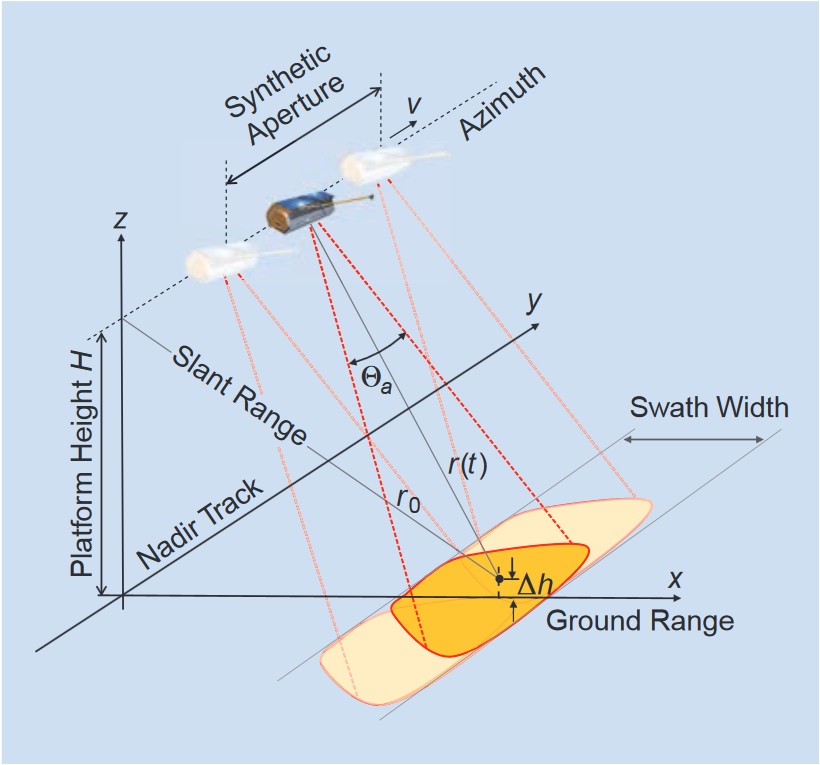
\includegraphics[width=0.8\linewidth]{Cap1-Bib-Review/geometry.png}
    \caption{Illustration of SAR flight geometry.. $r_0$ is the shortest distance to the target, $\Theta_a$ stands for the azimuth beamwidth, and $v$ for the satellite speed. \cite{tutorial}}
    \label{fig:SAR_geometry}
\end{figure}{}

Wavelength-resolution SAR systems are radar systems with resolution in the order of the system wavelength. When using wavelength-resolution SAR images to detect targets, it is important to mention that the size of the target matters to the final image registered. According to \cite{63}, SAR images of targets with dimensions of the order of the wavelength might present the resonance scattering phenomena, and targets that are small compared to the wavelength might present the Rayleigh scattering phenomena. 

One of the datasets used throughout this work was acquired with a wavelength resolution ultrawide-band (UWB) very-high frequency (VHF) SAR system.  For low-frequency (VHF) UWB SAR images, the scattering process is mainly related to large scatters. This kind of scatters tends to be stable in time and less influenced by environmental effects. Due to stability between the images, change detection methods are usually performed with the highest possible resolution without using any type of clutter reduction filtering.  

A relevant aspect of SAR images is the Speckle noise. According to \cite{63, 17}, speckle noise is mainly due to multiple targets reflecting the emitted pulses. However, since the size of targets for wavelength-resolution SAR is approximately the order of the wavelength and, therefore, close to the system resolution, there can be only one scatterer inside each resolution cell. Thus, for target detection using wavelength-resolution SAR, speckle noise is not the main cause of problems. Because of that, it is of great importance to choose an appropriate frequency when designing the SAR system since different system frequencies will be more or less adequate for detecting targets of different sizes.


\subsection{SAR Image Formation}
SAR image formation, also called SAR image synthesis, starts after registering the received echoes (raw data). The acquired raw data is not yet ready for interpretation and information extraction \cite{Alberto} and needs to be processed to obtain a SAR image, which is the product required for post-processing applications. The first step is to perform matched filter operations to enhance the received signal. This is done by convolving the received raw data with the reference signal in the azimuth and range directions. More details on SAR image synthesis are referred to \cite{Alberto, livro}. After processing the raw data, a complex image (with amplitude and phase information) called the single-look complex (SLC) matrix is obtained. The amplitude value of this image represents the power reflected. The backscatter --- analogous to the reflectivity --- of the scene can be obtained by multiplying the amplitude value by a calibration constant obtained experimentally. The backscatter is of great importance to interpreting the image since this information can be used to detect and classify objects on Earth's surface \cite{radiometric} since different objects present different backscatter characteristics.

According to \cite{Raney,Small}, it is also possible to define different backscatter measures. The backscatter value represents the reflectivity normalized by the area of incidence, which can be measured in different directions. A backscatter is measured in an area orthogonal to the range direction (which has area $A_\gamma$), and it is called gamma-naught ($\gamma^0$). It is also possible to normalize the reflectivity by the ground area, $A_\sigma$ --- the corresponding backscatter value is called sigma-naught ($\sigma^0$) --- or by the area $A_\beta$ in the plane formed by the range and azimuth directions --- the corresponding backscatter is called beta-naught ($\beta^0$). All these values are of importance, since they all can be used to characterize the scene and perform target detection and classification. The relationship between $\sigma^0$, $\gamma^0$, and $\beta^0$ is given by

\begin{equation}
    \sigma^0 = \gamma^0 \cdot \cos(\theta) = \beta^0 \cdot \sin(\theta),
\end{equation}

\noindent
where $\theta$ is the incidence angle of the emitted pulse. A visual description of these normalized backscatter coefficients is shown in \figref{fig:normalization_areas}

\begin{figure}[H]
    \centering
    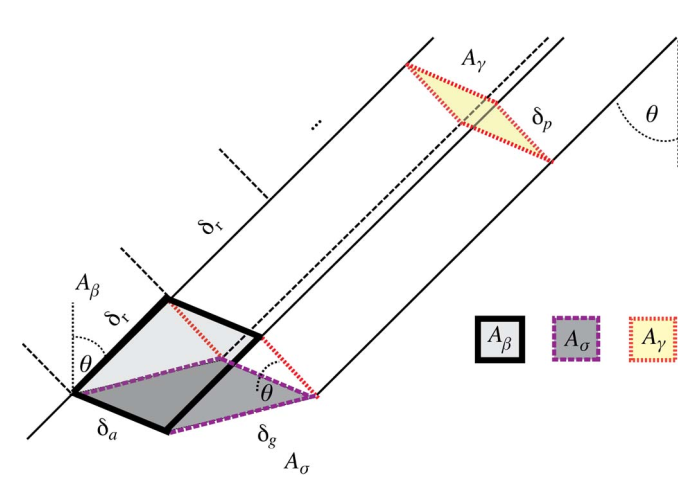
\includegraphics[width=0.8\linewidth]{Cap1-Bib-Review/retang.png}
    \caption{Normalization areas for SAR backscatter. \cite{Small}}
    \label{fig:normalization_areas}
\end{figure}

After obtaining the SLC image, it is also necessary to perform additional steps such as coregistration, geocoding, and calibration, among others, to obtain an image ready for visual interpretation. All those steps are outside the scope of this work. For the curious reader, it is referred \cite{Alberto} for more details on techniques used for SAR image processing. 

\subsection{Coherence SAR images}
A single SLC image is enough for classifying and detecting objects and scenarios on the Earth's surface, as can be seen in \cite{Paolathesis,Andreathesis, 78, 79, rfsar}. However, using more than one SLC image can favor classifying and detecting since adequate techniques are considered.  For example, when there are two images of the same area, it is possible to combine both images into a single image, called the ``interferometric coherence image.'' The coherence image can be computed by taking the complex correlation between the pairs of corresponding pixels of the two acquisitions, as follows

\begin{equation}
    \gamma = \frac{E[u_1u_2^*]}{\sqrt{E[|u_1|^2]E[|u_2|^2]}},
\end{equation}{}

\noindent
where $E[\cdot]$ is the expectation operator, $u_1$ is a pixel of the first image and $u_2$ is the corresponding pixel of the second image. One must keep in mind that it is not possible to compute the expected value since the probability density function (PDF) for the pixel is unknown. In practice, the correlation is computed using numerical estimations around the pixel of interest. For more details concerning the numerical estimation --- and the trade-offs between computing methods --- of the complex coherence, the reader is referred to \cite{Bamler}. After extracting the complex coherence (some sources use the term correlation/decorrelation instead of coherence) between pairs of images, the final result is an image that provides relevant information for classification and target identifying purposes as it can be seen in \cite{Alberto,Paolathesis,Martone, Martone2, Martone3, first_interferometric, Krieger,Paolo, Acqua}.

Multiple factors can affect the final coherence image, and some are relevant for the final result of this work. In \cite{Krieger,Paolathesis}, there is a detailed explanation concerning the coherence factors, but for this work, only two coherence factors matter:
\begin{enumerate}
    \item $\gamma_{Temp}$: Is the coherence factor due to the temporal baseline between both acquisitions. The longer the time separation between the two images, the more degraded the final coherence image will be due to this temporal coherence factor.
    \item
    $\gamma_{Vol}$: is the volume correlation factor, and it is due to volume scattering (scattering caused by multiple scatters inside the same resolution cell). On forests this is mainly due to vegetation and therefore is crucial for forest land-cover classification.
\end{enumerate} 

The temporal and volumetric coherences are crucial for the creation of land cover classification maps, as can be seen in \cite{Paolo, Rodrigo}, so the reader is referred to these works to understand better the applications and models used for the creation of land cover maps from coherence images.

\section{SAR Images for Land Cover Classification Maps}

Land Cover maps are maps that measure the area and perimeter of different field types
on the Earth's surface. Since land coverage maps have broad applications - ranging from
environmental, economical and ecological purposes - it is important that the accuracy
be as high as possible. Since it is not feasible to physically measure the environmental
degradation of a forest (because this does not scale well to large areas), normally these
measurements are done with remote sensing data. The GlobCover \cite{globcover, glob} (European Space Agency GlobCover Portal) map is one example
of a classification map that was generated using MERIS data. Regarding coverage maps, there are mainly three areas of interest: vegetated areas, deforested areas, and artificial surfaces (human-made surfaces like constructions, buildings, roads, landmarks, houses, etc.). Among these areas, they can be further divided into subclasses. For example, vegetated areas can be further divided into irrigated croplands, deciduous forests, and mosaic grassland. This is the standard used by the Glob-Cover map and many other land coverage maps. Figure \ref{fig:glob_cover_map} shows a Glob-Cover map created in 2018. 


\begin{figure}[H]
    \centering
    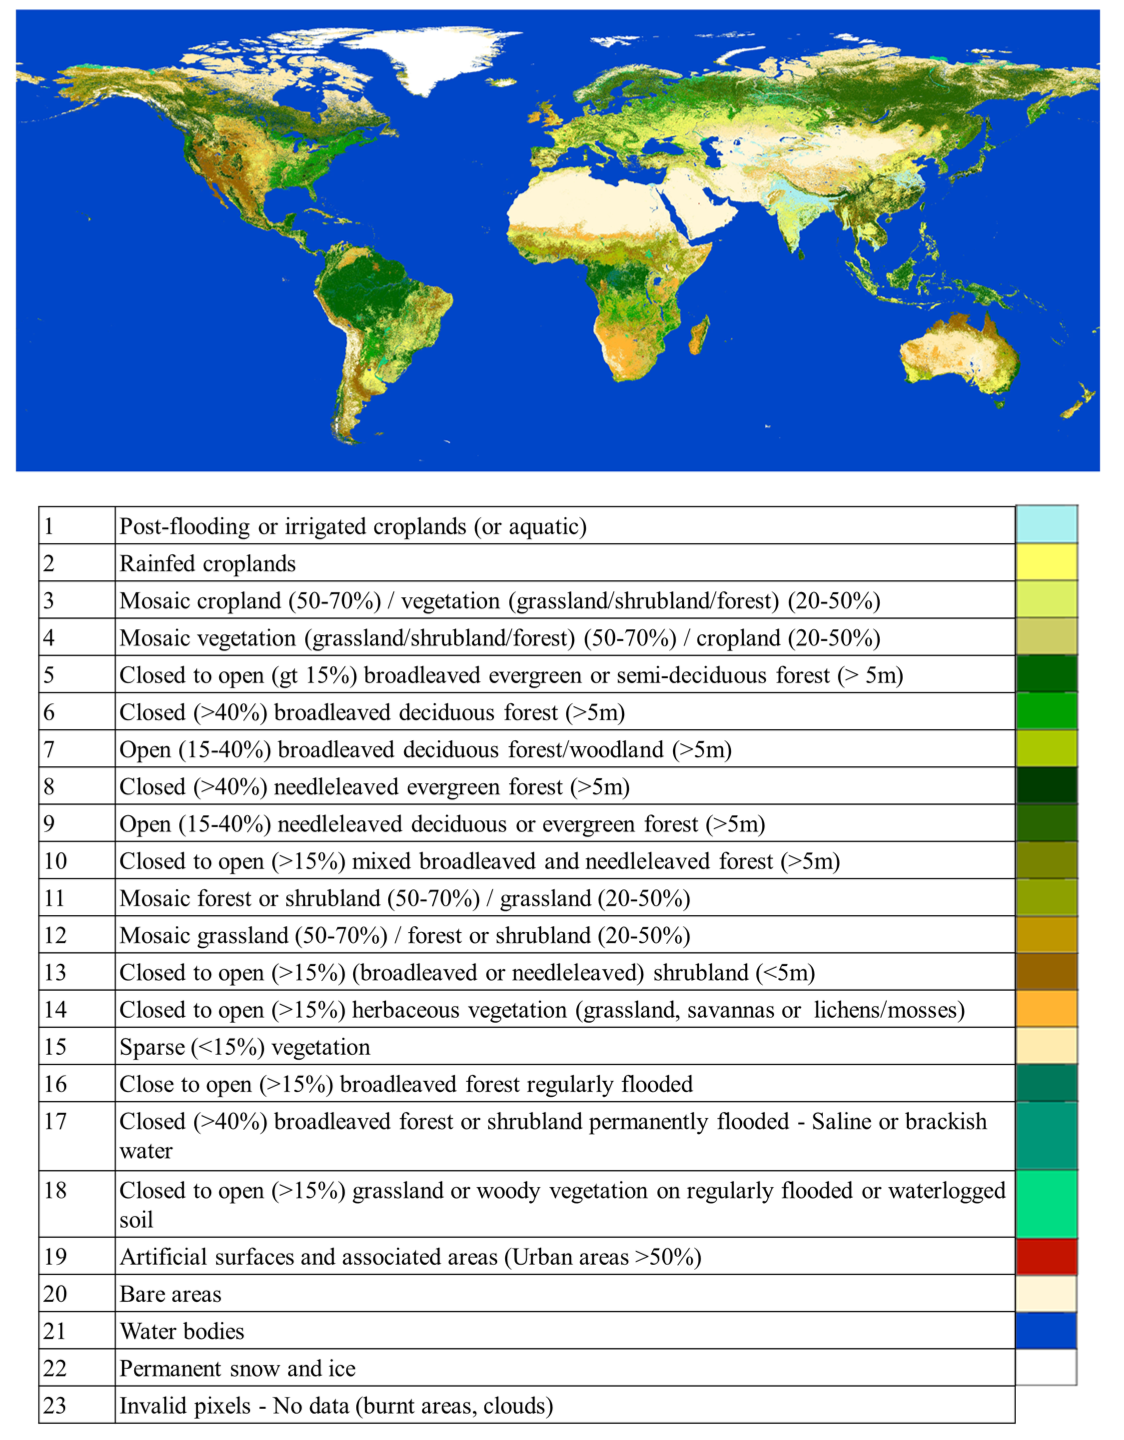
\includegraphics[width=\linewidth]{Cap2/glob_cover.png}
    \caption{GlobCover classification map \cite{Paolathesis}.}
    \label{fig:glob_cover_map}
\end{figure}

GlobCover map is created using optical sensors. This method can easily generate a classification from the optical data. However, it has the disadvantage of being weather dependent and cannot provide high-resolution maps. SAR land coverage maps have none of these disadvantages, but it comes at the price that it is harder to create an accurate classification map.

The L-Band ALOS PALSAR \cite{alos1, alos2, alos3,alos4, alos5, alos6} is a global coverage map created from SAR acquisitions based only on creating thresholds on the cross-polarization levels of the detected backscatter. Several forest maps were created for the Amazon rainforest and other tropical forests using ALOS PALSAR data. The coverage maps generated from ALOS PALSAR data present high classification accuracy and therefore are used for practical purposes. Even though it is possible to create land coverage maps based only on the backscatter measurement, it is possible to use the coherence information to further improve the accuracy results. \cite{first_interferometric} was the first reported case of forest coverage map created using coherence information. This work was done using ERS-1 SAR data and proved that not only forests can be clearly discriminated from other land categories, but it also showed that it is possible to distinguish among different forests types. By analyzing statistical properties of the coherence values of the area (such as mean and standard deviation) it was possible to infer which class that specific pixel belongs to. In \figref{fig:first_interferometric_estimate} it can be seen the statistical properties of coherence for different classes.

\begin{figure}[H]
    \centering
    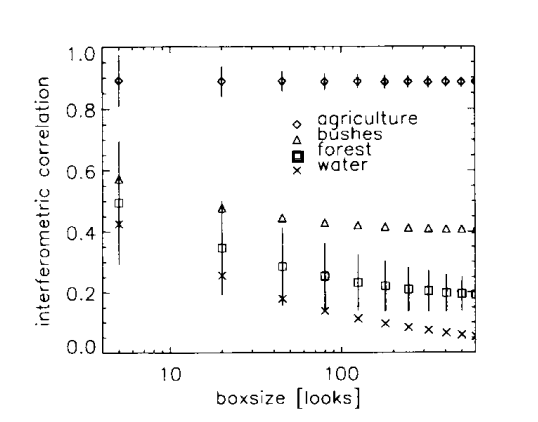
\includegraphics[width=0.7\linewidth]{Cap2/first_interferometric.png}
    \caption{Mean and Standard deviation of the coherence estimate as number of looks (filter size) for different classes \cite{first_interferometric}.}
    \label{fig:first_interferometric_estimate}
\end{figure}

This thesis proposes new approaches to explore the backscatter and coherence statistical properties based on the ideas presented in \cite{first_interferometric}; however, with more significant results due to the available computational power today. Both techniques, i.e., x and y, were combined to improve the accuracy of the land cover classification maps. The backscatter information is combined with the coherence information to achieve a maximum accuracy land coverage map. The classification algorithm presented in this thesis was inspired in the techniques presented in \cite{Paolathesis,Paolo, Martone, Martone2, Martone3, Rizzoli}. 

\section{Change Detection Algorithms}
When working with SAR systems, multi-temporal acquisitions of the same area might be performed, i.e., acquisitions of the same ground area obtained with a temporal baseline. Multi-temporal images can be used for information extraction in two ways: i) accessing the information contained in the entire time frame, or ii) accessing the difference between images \cite{change1}. Change detection in remotely sensed data may be done in a supervised or unsupervised way. Supervised techniques require that a ground truth be available to derive a training set for the training process of the detectors. Meanwhile, unsupervised methods do not require ground truth data \cite{change2,change3}. Since the creation of ground truths is a very time-demanding task, unsupervised change detection algorithms are usually performed. Still, they come with the disadvantage that unsupervised algorithms underperform when compared to supervised algorithms.

Change detection can be seen as a particular case of a multi-temporal image classification problem. Typically, change detection algorithms are considered for either pre-classification or post-classification approaches. In pre-classification algorithms, pairs of images are inputs, and the outputs are labeled images. Then another algorithm uses the labeled images to identify the pixel labels that have changed. In post-classification, a single classification is performed directly on the combined image-pair dataset \cite{change4}. 

Even though there are multiple approaches and algorithms for change detection, most of them dwell on two problems \cite{change5}:
\begin{enumerate}
    \item Creating a change measure or change indicator image
    \item Thresholding the change indicator values to produce a binary change map.
\end{enumerate}

Several measures can be used to detect change. Usually, the change measure used is based on the ratio or the log ratio of two images \cite{change6}. However, plenty of other measures can be used as change measures, e.g., mean-ratio operator, triplet Markov field model measure, Radon transform, Jeffrey divergence, Garbor functions, and power spectrum of the image, among others \cite{change5, change6, change7}. Even though most of the change measures are related to the post-processed and filtered images, some techniques rely on the noise and speckle of the image. One prominent approach that shows high accuracy is based on modeling the speckle of the image as a fractional Brownian motion and as a fractal image, extracting information concerning the Brownian motion and the fractal dimension of the image and using this value to create the change measure for classification \cite{change5}.

After creating the change measure, the only step left is detecting the changes. Traditional CDAs are based on standard statistical theory, e.g., traditional hypothesis testing, such as the generalized likelihood ratio test \cite{GLRT1,GLRT2,GLRT3}, maximum a posteriori test \cite{Book_Kay}, Bayesian theory approaches \cite{Bayes1, Bayes2}, or likelihood ratio test \cite{LRT1,LRT2,LRT3}. Most of these methods perform adequately in terms of probability of detection, but most show poor performance in terms of false alarm rate \cite{Carabas,Ricardo,LucasRamos,Chris}. Those methods also have other drawbacks, such as dependency on morphological operations (erosion and dilation filters) and algorithm calibration for new data sets.

Machine learning algorithms have become popular in the last few years \cite{Vinholi, Campos} since they can perform better than statistical-based CDAs and do not have drawbacks the ordinary methods present. There are two main types of machine learning algorithms: supervised and unsupervised. Supervised algorithms have a classification reference to help guide the learning step, while unsupervised algorithms do not have a classification reference. In this dissertation, we focused only on supervised algorithms. Generally, CD algorithms are assessed considering the following metrics: i) the number of true positives, ii) the number of true negatives, iii) the number of false positives, and iv) the number of false negatives \cite{PefMe}. For this thesis, the parameters of interest are the number of true positives and false negatives.

Among the supervised machine learning algorithms, there are many options for the applications considered in this thesis. These include Neural Networks, Naive Bayes, Linear Regression, Kernel Ridge Regression, Support Vector Machine, Decision Trees, and Random Forest \cite{PefMe}. For this work, it is used a neural network-based algorithm. There are multiple types of neural networks, e.g., perceptron, Feed Forward Neural Network, Multilayer Perceptron, Recurrent Neural Network, Long Short-Term Memory Neural Network, and convolutional neural network, among others \cite{PefMe}. We decided to use a UNET convolutional neural network \cite{Unet} to solve the target detection problem since CNNs have provided excellent results for computer vision problems. In \cite{Kevin}, a similar approach was used to detect changes in X-band SAR images. 

In this work, it is proposed a new approach that combines pre- and post-classification techniques. The technique chosen for the classification method is a UNET CNN-based network to create the final change detection map. The UNET CNN uses SAR images as input for the target detection, but also textural information is explored according to the method. The textural information extraction technique is used on the pre-classification step, and this information will be used to improve the results of the post-classification step that will be performed by the UNET. In \cite{Rodrigo}, it was already shown that additional textural information could provide valuable information to improve classification results. It is important to mention that since CNN uses convolutions, which are linear filters, to achieve better classification results, it would be redundant to use linear textural information as inputs to the UNET CNN. When comparing the proposed technique with other algorithms on the same dataset, we show that the results show similar detection performance but significant improvement in false alarm rate.

